\section{Synthesis and test on FPGA}
\subsection{Measure area and performance}
\todo[inline]{Make a table with output from viavdo and server}
%\inputminted[linenos=0, firstline=82, lastline=102, frame=none]{text}{../RSA/synthesis_report.txt}
%\inputminted[linenos=0, firstline=309, lastline=318, frame=none]{text}{../RSA/synthesis_report.txt}
%
\begin{table}[htp]
    \begin{center}
        \begin{tabular}{l | r}
            Instance                     & Cells \\
            \hline
            Total RSA                    & 2833 \\
            \quad monpro                 & 1428 \\
            \qquad u\_monpro\_controller & 293  \\
            \qquad u\_monpro\_datapath   & 1135 \\
            \quad u\_rsa\_controller     & 74   \\
            \quad u\_rsa\_datapath       & 1261 \\
        \end{tabular}
        \caption{Cell usage divided by instances}
        \label{tab:cell_usage}
    \end{center}
\end{table}

\begin{table}[htp]
    \begin{center}  
        \begin{tabular}{ l | c | c | r}
             Resource & Utilization & Available & Utilization \%  \\
             Slice LUTs & 1024 & 218600 & 0.47 \\
             Slice Registers & 1245 & 437200 & 0.28 \\
             IO & 69 & 362 & 19.06 \\
             Clocking & 1 & 32 & 3.12 \\
        \end{tabular}
        \caption{Summary of resource utilization }
        \label{tab:resource_utilization}
    \end{center}
\end{table}
%
\begin{figure}[htp]
    \centering
    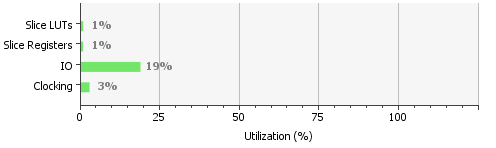
\includegraphics[width=0.6\textwidth]{images/utilization}
    \caption{A graph over the utilization of the various resources}
    \label{fig:utilization}
\end{figure}

\subsection{Prove that the design actually works on FPGA}
\inputminted[linenos=0]{text}{../rocket.txt}
%
\subsection{Discuss/Analyze/Conclude}